\section{Connectedness}
\label{connectedness}
In $\bbR^n$, we have a good intuition about what it means for subsets to be connected or not. For example, the subset $[-2,-1] \cup [1,2]$ does seem very connected: how would we connect $-1$ and $1$? On the other hand, a set $(-2,2)$ should probably deserve to be called connected.

It turns out that having open sets is sufficient to define a notion of connectedness that agrees with out intuition in the intuitive examples; this is the subject of this sections.

\subsection{Connectedness}
\begin{defn}
  Let $X$ be a topological space. A \word{separation}{?} of $X$ is a pair $U$, $V$ of disjoint non-empty open subsets of $X$ so that $X = U \cup V$. We say that $X$ is \word{connected}{sammanh{\"a}ngande} if it has no separation.
\end{defn}
\trans{separation}{?}\trans{connected}{sammanh{\"a}ngande}
In the following we will often be dealing with connectedness of subspaces. Keep in mind that when doing so, the subspace will always be equipped with the subspace topology.
\begin{example}
  The subspace $(-2,-1) \cup (1,2) \subset \bbR$ has a separation.
\end{example}
Notice that if $X = U \cup V$ is a separation, then $U = X \setminus V$ and $V = X \setminus U$. This means that both $U$ and $V$ are both open and closed.
\begin{lem}
  A topological space $X$ is connected if and only if $\emptyset$ and $X$ are the only subsets of $X$ that are both open and closed.
\end{lem}
\begin{proof}
  Suppose that $U \subset X$ is both open and closed. Then $V = X \setminus U$ is open, and $X = U \cup V$ is a separation. If $X$ is connected one of $U$ and $V$ must be empty, since otherwise we would have a separation of $X$.
\end{proof}
% \begin{lem}
%   A topological space $X$ is connected if and only if the following condition holds: if $X = C \cup D$ where $C$ and $D$ are disjoint closed subsets of $X$, then either $C = \emptyset$ or $D = \emptyset$.
% \end{lem}
% \begin{proof}
%   Exercise.
% \end{proof}
\begin{example}
  The rational numbers $\bbQ \subset \bbR$ are not connected: choose any irrational number $a \in \bbR$. Then
  \[
    \bbQ = ((-\infty, a) \cup (a,\infty)) \cap \bbQ = ((-\infty,a) \cap \bbQ) \cup (\bbQ \cap (a,\infty)),
  \]
  which is a separation by definition of the subspace topology on $\bbQ$.
\end{example}
\begin{example}
  \label{discrete-connectedness}
  If $X$ has the discrete topology and consists of more than two points, then $X = \{x\} \cup (X \setminus \{x\})$ is a separation of $X$, so $X$ is not connected.
\end{example}
\begin{example}
  \label{intervals-are-connected}
  Let $I \subset \bbR$ be any interval (bounded, unbounded, open, closed, or half-open). We claim that $I$ is connected. We will use the (hopefully) well-known fact that any subset $A \subset \bbR$ satisfies $\sup A \in \bar A$ (since, for instance, $\sup A$ is a limit of a sequence in $A$ so that we can use Lemma~\ref{closure-convergence}).
  
  Now to see the claim, assume that $I = U \cup V$ is a separation of $I$, let $x \in U$, $y \in V$, and assume without loss of generality that $x < y$. Then we have $[x,y] \subset I$. Let $U_0 = [x,y] \cap U$, $V_0 = [x,y] \cap V$ so that $[x,y] = U_0 \cup V_0$ is a separation of $[x,y]$, and define $z = \sup U_0 \in [x,y]$. Now as noticed above, $U_0$ is both open and closed in $[x,y]$ so in particular $U_0$ is also closed in $\bbR$, so $z \in \bar{U_0} = U_0$. If $z = y \in V_0$, we have a contradiction, so assume that $z \not= y$. Since $U_0$ is open in $[x,y]$ we can find $u \in U_0$ so that $z < u$, which contradicts the fact that $z = \sup U_0$ (to be completely precise about this last point, $U_0 = [x,y] \cap U_1$ for an open set $U_1 \subset \bbR$, and we can find a neighbourhood $B(z,r)$ of $z \in U_1$ so small that $B(z,r) \subset U_0$; we now just take $u = z+r/2$).
  
  On the other hand, one can show that if $I \subset \bbR$ is connected, then $I$ is an interval (this is Exercise~\ref{connected-implies-interval}).
\end{example}
\begin{rem}
  Being connected is a topological property which can be used to define a simple topological invariant: if $X$ is connected any $Y$ is not, then $X$ and $Y$ are not homeomorphic.
\end{rem}
\begin{lem}
  \label{connectedness-subspace-lemma}
  Let $X = U \cup V$ for disjoint open sets $U$ and $V$, and let $Y \subset X$ be a subspace. If $Y$ is connected, then $Y \subset U$ or $Y \subset V$.
\end{lem}
\begin{proof}
  We will show the contrapositive of the statement, so assume that $Y \cap U \not= \emptyset$ and $Y \cap V \not= \emptyset$. Then
  \[
    Y = Y \cap X = Y \cap (U \cup V) = (Y \cap U) \cup (Y \cap V)
  \]
  is a separation of $Y$, since $Y \cap U$ and $Y \cap V$ are disjoint, non-empty and open in the subspace topology. Thus $Y$ is not connected.
\end{proof}
\begin{thm}
  \label{unions-connected}
  Let $\{A_i\}_{i \in I}$ be a collection of connected subspaces of a topological space $X$ with a common point $x \in X$; i.e. $x \in A_i$ for all $i \in I$. Then $\bigcup_{i \in I} A_i$ is connected.
\end{thm}
\begin{proof}
  Suppose that $\bigcup_{i \in I} A_i = U \cup V$ for disjoint subsets $U$ and $V$ that are open in $\bigcup_{i \in I} A_i$ and let us show that either $U$ or $V$ must be empty. Assume without loss of generality that $x \in U$. By Lemma~\ref{connectedness-subspace-lemma} we have for each $i$ that either $A_i \subset U$ or $A_i \subset V$. Since $x \in A_i$ we must have $A_i \subset U$ for all $i \in I$. This implies that $\bigcup_{i \in I} A_i \subset U$, so $V$ must be empty.
\end{proof}
\begin{thm}
  \label{connected-closures}
  Let $A \subset X$ be connected. If a subset $B \subset X$ satisfies $A \subset B \subset \bar A$, then $B$ is also connected. In particular, $\bar A$ is connected when $A$ is.
\end{thm}
\begin{proof}
  Suppose that $B = U \cup V$ for disjoint subsets $U$ and $V$ that are open in $B$. Then by Lemma~\ref{connectedness-subspace-lemma} we must have that $A \subset U$ or $A \subset V$, so assume without loss of generality that $A \subset U$. Then $B \subset \bar A \subset \bar U$ (where all closures are in the bigger space $X$).
  
  By definition of the subspace topology, there are open sets $U'$ and $V'$ in $X$ so that $U = B \cap U'$, $V = B \cap V'$, and
  \[
    U = B \setminus V = B \setminus (B \cap V') \subset X \setminus V'.
  \]
  The latter space is closed so $\bar U \subset X \setminus V' \subset X \setminus V$. Putting this together, $B \subset X \setminus V$ which means that $B \cap V = \emptyset$, so $V = \emptyset$, and so $B$ is connected.
\end{proof}
\begin{thm}
  \label{images-of-connected}
  Let $f : X \to Y$ be a continuous map between two topological spaces. If $X$ is connected, then $f(X)$ is also connected.
\end{thm}
\begin{proof}
  Suppose that $f(X) = U \cup V$ for disjoint subsets $U$ and $V$ that are open in $f(X)$. Then $f^{-1}(U)$ and $f^{-1}(V)$ are disjoint open subsets of $X$ with $X = f^{-1}(U) \cup f^{-1}(V)$. This means that either $f^{-1}(U)$ or $f^{-1}(V)$ is empty. Suppose that $f^{-1}(U)$ is empty. Then since $U \subset f(X)$ we must have $U = \emptyset$.
\end{proof}
\begin{cor}
  Let $X$ be a connected topological space, and let $Y$ be any set. Suppose that $f : X \to Y$ is a locally constant\index{locally constant} map, meaning that every point $x \in X$ has a neighbourhood $U$ so that $f|_U$ is constant. Then $f$ is constant.
\end{cor}
\begin{proof}
  Give $Y$ the discrete topology. Then the condition that $f$ is locally constant implies that $f$ is continuous at every point, so $f$ is continuous. Thus $f(X)$ is connected by Theorem~\ref{images-of-connected}, but $f(X)$ also has the discrete topology, so by Example~\ref{discrete-connectedness} it consists of a single point which is the same as saying that $f$ is constant.
\end{proof}
\begin{cor}[Intermediate value theorem]
  \index{intermediate value theorem}Let $f : X \to \bbR$ be continuous and assume that $X$ is connected. If there is an $r \in \bbR$ and $x,y \in X$ so that $f(x) < r < f(y)$, then there is a $z \in X$ with $f(z) = r$.
\end{cor}
\begin{proof}
  By Theorem~\ref{images-of-connected}, $f(X)$ is connected, thus an interval by Exercise~\ref{connected-implies-interval}. Since $f(x),f(y) \in f(X)$, we therefore have $r \in [f(x),f(y)] \subset f(X)$.
\end{proof}
\begin{thm}
  \label{products-connected}
  If $\{X_i\}_{i \in I}$ is a family of topological spaces, then their product $\prod_{i \in I} X_i$ is connected if and only if every $X_i$ is.
\end{thm}
\begin{proof}
  Suppose that the product is connected. Recall that the projection $\pi_j : \prod_{i \in I} X_i \to X_j$ is continuous for every $j$, so every $X_j$ is connected by Theorem~\ref{images-of-connected}.
  
  Let us show the converse in the case where $I$ is finite. The infinite case is left as Exercise~\ref{exercise-products-connected}. Moreover, we can reduce to the case $\abs{I} = 2$ by induction since $(X_1 \times \cdots X_{n-1}) \times X_n \simeq X_1 \times \cdots X_n$, which is not difficult to show.
  
  Thus, we are left to show that $X \times Y$ is connected when $X$ and $Y$ are. We will write $X \times Y$ as a union of connected spaces with a common point and use Theorem~\ref{unions-connected}. For any point $x \in X$, we let $A_x = \{x \} \times Y$. Then $A_x$ is the image of the map $Y \to X \times Y$ given by $y \mapsto (x,y)$, so $A_x$ is connected by Theorem~\ref{images-of-connected}. Similarly one shows that $B_y = X \times \{y\}$ is connected for all $y \in Y$. By Theorem~\ref{unions-connected}, $A_x \cup B_y$ is connected for all $y \in Y$ since $(x,y)$ is contained in both $A_x$ and $B_y$. Now clearly,
  \[
    X \times Y = \bigcup_{y \in Y} A_x \cup B_y,
  \]
  and all the sets on the right hand side have the common point $(x,y') \in A_x$, where $y' \in Y$ can be taken to be anything. Therefore, their union is connected by Theorem~\ref{unions-connected}.
\end{proof}
Since we have seen that $\bbR$ is connected, we immediately obtain the following.
\begin{cor}
  Euclidian space $\bbR^n$ is connected for any $n \in \bbN$.
\end{cor}
\begin{prop}
  The $n$-sphere $S^n$ and the $n$-torus $T^n$ are connected for all $n \in \bbN$.
\end{prop}
\begin{proof}
  If we can show that $S^1$ is connected, then so is $T^n = S^1 \times \cdots \times S^1$ for all $n \geq 1$.
  
  Let us show that $S^n$ is connected. Recall from Proposition~\ref{north-pole-removed} that $S^n \setminus \{p\} \simeq \bbR^n$, where $p$ is the north pole. It follows that $S^n \setminus \{p\}$ is connected. Now one can show that $\bar{S^n \setminus \{p\}} = S^n$ and so the result follows from Theorem~\ref{connected-closures}.
\end{proof}
Alternatively, one can show that $\bbR^{n+1} \setminus \{0\}$ is connected when $n \geq 1$ (Exercise~\ref{origin-removed-connected}); then the connectedness of $S^n$ follows because $S^n$ is the image of the continuous map $f : \bbR^{n+1} \setminus \{0 \} \to \bbR^{n+1}$ given by $f(x) = x/\Abs{x}$.

The following is an example of how to use connectedness as a topological invariant:
\begin{prop}
  For any $n \in \bbN$, we have $S^n \not\simeq \bbR$.
\end{prop}
\begin{proof}
  Suppose that we had a homeomorphism $f : S^n \to \bbR$. Then $f$ would restrict to a homeomorphism if we removed the north pole $p$ from $S^n$; that is, $f|_{S^n \setminus \{p \}} : S^n \setminus \{p\} \to \bbR \setminus \{f(p)\}$ is a homeomorphism. This implies that $\bbR^n \simeq S^n \setminus \{p\} \simeq \bbR \setminus \{f(p)\}$, but $\bbR^n$ is connected while $\bbR \setminus \{f(p)\}$ is not connected, so they can not be homeomorphic, and we obtain a contradiction.
\end{proof}

Along the same lines, we mention the following result.
\begin{thm}[Brouwer's invariance of dimension]
  \label{invariance-of-dimension}
  \index{Brouwer's invariance of dimension}If two non-empty open sets $U \subset \bbR^n$ and $V \subset \bbR^n$ and $U \simeq V$, then $n = m$.
\end{thm}
The proof uses methods from algebraic topology and will not be covered here; see e.g. \cite[Thm.~2.26]{Hat}. A special case is contained in Exercise~\ref{invariance-of-dimension-exercise}.


\subsection{Paths and path-connectedness}
Another natural notion of connectedness is obtained by requiring that all points in a space can be connected to each other; what exactly to mean by this is contained in the following definition.

\begin{defn}
  Given two points $x$ and $y$ in a topological space $X$, a \word{path}{?} from $x$ to $y$ is a continuous map $\gamma : [0,1] \to X$ so that $\gamma(0) = x$, $\gamma(1) = y$. If for any pair $x,y$ in $X$ there is a path from $x$ to $y$, we say that $X$ is \word{path-connected}{b{\aa}gvis sammanh{\"a}ngande}.
\end{defn}
\trans{path}{?}\trans{path-connected}{b{\aa}gvis sammanh{\"a}ngande}
\begin{prop}
  \label{path-connected-implies-connected}
  A path-connected space is connected.
\end{prop}
\begin{proof}
  We will prove the contrapositive, so let $X = U \cup V$ be a separation of $X$. Suppose that $\gamma : [0,1] \to X$ is any path. Then by Example~\ref{intervals-are-connected} and Theorem~\ref{images-of-connected} we see that $\gamma([0,1])$ is connected and by Lemma~\ref{connectedness-subspace-lemma}, $\gamma([0,1])$ is contained entirely in $U$ or in $V$. This means that it is not possible to find paths from points in $U$ to points in $V$.
\end{proof}
\begin{example}
  For $x, y \in \bbR^n$, the path $\gamma : [0,1] \to \bbR^n$ defined by
  \[
    \gamma(t) = (1-t)x + ty
  \]
  is a path from $x$ to $y$, so $\bbR^n$ is path-connected.
\end{example}
\begin{example}
  A subset $A$ of $\bbR^n$ is called convex if for any $x,y \in A$, the image of the straight line $\gamma(t) = (1-t)x + ty$ belongs to $A$. As in the previous example, it follows that convex subsets are path-connected and thus also connected.
  
  Some examples of convex subsets are the upper half-plane
  \[
    \{(x_1,\dots,x_n) \in \bbR^n \mid x_n > 0\}
  \]
  and any ball $B(x,r)$, $x \in \bbR^n$, $r > 0$.
\end{example}
\begin{example}
  A connected space does not need to be path-connected. A counter-example is the so-called topologist's sine curve
  \[
    S = \{(x,y) \in \bbR^2 \mid y = \sin(1/x), x > 0 \} \cup \{(0,y) \mid -1 \leq y \leq 1 \},
  \]
  that is, the closure of the graph of $x \mapsto \sin(1/x)$ for $x > 0$; see Figure~\ref{sinecurve}. For details, see \cite[\S 24]{Mun}.
  \begin{figure}
    \centering
    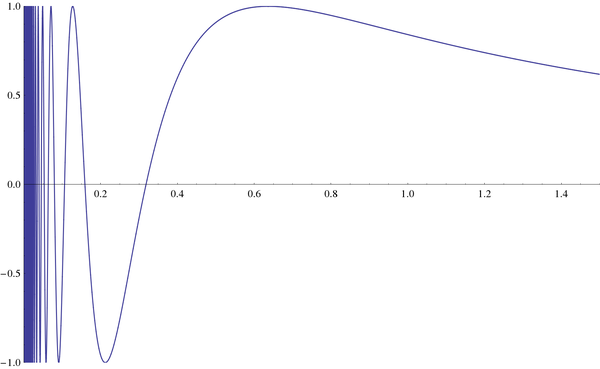
\includegraphics[width=.6\linewidth]{images/sinecurve}
    \caption{The topologist's sine curve.}
    \label{sinecurve}
  \end{figure}
\end{example}
On the other hand, the following result provides a necessary and sufficient condition for a connected space to be path-connected.
\begin{defn}
  A topological space $X$ is called \emph{locally (path-)connected at $x \in X$} if every neighbourhood of $x$ contains a (path-)connected neighbourhood of $x$. If $X$ is locally (path-)connected at each point $x \in X$, we say that $X$ is \word{locally (path-)connected}{lokalt (b{\aa}gvis) sammanh{\"a}ngande}.
\end{defn}
\trans{locally (path-)connected}{lokalt (b{\aa}gvis) sammanh{\"a}ngande}
\begin{thm}
  \label{path-connected-vs-connected}
  A topological space is path-connected if and only if it is connected and locally path-connected.
\end{thm}
One direction follows immediately from Proposition~\ref{path-connected-implies-connected}. For the other, it will be useful to have at our disposal the notion of connected components.

\subsection{Connected components and path-connected components}
\label{component-section}
Recall that the subset $(-2,-1) \cup (1,2) \subset \bbR$ was not connected. It does however have two natural subspaces, $(-2,1)$ and $(1,2)$ which \emph{are} connected. We will now see how to split every topological space into connected parts.

\begin{prop}
  Let $X$ be a topological space. Define a relation $\sim$ by on $X$ by declaring that $x \sim y$ if and only if there is a connected set $A \subset X$ so that $x,y \in A$. Then $\sim$ is an equivalence relation. The equivalence classes of $\sim$ are called the \wordexp{connected components}{sammanh{\"a}ngande komponenter}{connected component}{sammanh{\"a}ngande komponent} of $X$.
\end{prop}
\trans{connected component}{sammanh{\"a}ngande komponent}
\begin{proof}
  We see that $x \sim x$ for every $x$, since $\{x\}$ is connected.
  
  If $x \sim y$ there exists a connected set $A$ with $x,y \in A$. Then clearly $y,x \in A$ so $y \sim x$.
  
  If $x \sim y$ and $y \sim z$ we get connected sets $A$, $B$ so that $x,y \in A$ and $y,z \in B$. Let $C = A \cup B$. Then $x,z \in C$, and $C$ is connected by Theorem~\ref{unions-connected}, so $x \sim z$.
\end{proof}
\begin{prop}
  \label{props-of-conn-components}
  Let $\{C_i\}_{i \in I}$ be the set of connected components of a topological space $X$. Then
  \begin{itemize}
    \item[(i)] $X = \bigcup_{i \in I} C_i$ and the $C_i$ are pairwise disjoint,
    \item[(ii)] if $Y \subset X$ is connected, then $Y \subset C_i$ for some $i \in I$,
    \item[(iii)] $C_i \subset X$ is connected for each $i \in I$
    \item[(iv)] $C_i$ is closed for all $i \in I$.
  \end{itemize}
\end{prop}
\begin{proof}
  The first part is trivial since it it always true for equivalence classes of an equivalence relation. Let $Y \subset X$ be connected, and let $x \in Y$. Then $y \in [x]$ for all other $y \in Y$ since $Y$ is a connected set containing both $x$ and $y$, so $Y \subset [x]$, and $[x]$ is one of the $C_i$ by definition.
  
  Similarly, fix $x \in C_i$. Then for every other $y \in C_i$ there a connected subset $A_y$ so that $x, y \in A_y$. Then $A_y \subset C_i$ by (ii), and we now use our usual trick and find that $C_i = \bigcup_{y \in C_i} A_y$. Since all of the $A_y$ contain $x$, we use Theorem~\ref{unions-connected} to conclude that $C_i$ is connected.
  
  Finally, we will show that $C_i$ is closed by showing that $C_i = \bar{C_i}$. Once more, write $C_i = [x]$ for any $x \in C_i$. Let $y \in \bar{C_i}$. Then $\bar{C_i}$ is a subset containing both $x$ and $y$, and $\bar{C_i}$ is connected by Theorem~\ref{connected-closures}, so $y \in [x] = C_i$.
\end{proof}
\begin{example}
  It follows from Proposition~\ref{props-of-conn-components} that connected components are open if there are only finitely many of them. This need not be the case though: we claim that the connected components of $\bbQ$ are the singleton sets $\{x\}$. Indeed, let $X$ be any subset of $\bbQ$ containing at least two points, and suppose that $x, y \in X$, $x \not= y$. There there is an irrational number $r$, $x < r < y$, and 
  \[
    X = (X \cap (-\infty,r)) \cup (X \cap (r,\infty))
  \]
  is a separation of $X$. We have already seen that the topology on $\bbQ$ is not the discrete one, so the connected component $\{x\}$ is not open for any $x$.
\end{example}
\begin{rem}
  The number of connected components is a topological invariant $\mathbf{Top} \to \bbZ \cup \{\infty\}$. That is, if two topological spaces have a different number of connected components, then they can not be homeomorphic.
\end{rem}

We now turn back to our study of path-connected spaces, creating an analogous construction of path-connected components. For this, it will first be useful to introduce the following two operations on paths. For any path $\gamma : [0,1] \to X$ in a topological space $X$, define the \emph{reverse}\index{reverse} of $\gamma$, denoted $\gamma^\inv$, by $\gamma^\inv(t) = \gamma(1-t)$. Then $\gamma^\inv$ is continuous, and if $\gamma$ is a path from $x$ to $y$, then $\gamma^\inv$ is a path from $y$ to $x$. Let $\gamma_1,\gamma_2 : [0,1] \to X$ be two paths so that $\gamma_1(1) = \gamma_2(0)$, so that $\gamma_1$ is a path from $x$ to $y$, and $\gamma_2$ is a path from $y$ to $z$. We then form a path from $x$ to $z$ as follows: define the \word{concatenation}{konkatenering} $\gamma_1 \star \gamma_2$ by
\[
  \gamma_1 \star \gamma_2(t) = \begin{cases} \gamma_1(2t), & t \in [0,\tfrac{1}{2}],\\ \gamma_2(2t-1), & t \in [\tfrac{1}{2},1]. \end{cases}
\]
We need to check that $\gamma_1 \star \gamma_2$ is actually continuous. This, however follows directly from the closed-set version of the pasting lemma, see Remark~\ref{pasting-closed}, applied to the two intervals $[0,\tfrac{1}{2}]$ and $[\tfrac{1}{2},1]$.

With this, we can define a relation on $X$ by saying that $x \sim_{\mathrm{path}} y$ if there is a path from $x$ to $y$.
\begin{lem}
  The relation $\sim_{\mathrm{path}}$ is an equivalence relation. The equivalence classes of $\sim_{\mathrm{path}}$ are called the \wordexp{path-connected components}{b{\aa}gvis sammanh{\"a}ngande komponenter}{path-connected component}{b{\aa}gvis sammanh{\"a}ngande komponent} of $X$.
\end{lem}
\trans{path-connected component}{b{\aa}gvis sammanh{\"a}ngande komponent}
\begin{proof}
  The constant path $\gamma:[0,1]\to X$, $\gamma(t) = x$, is continuous for any given $x \in X$, so $x \sim_{\mathrm{path}} x$. The other conditions for an equivalence relation are obtained by using the operations on paths introduced above.
\end{proof}

We have the following analogue of Proposition~\ref{props-of-conn-components} for path-connected components; its proof is similar and omitted.
\begin{prop}
  \label{prop-path-connected-components}
  The path-connected components are path-connected disjoint subspaces of $X$ whose union is $X$. If a subspace is path-connected, it is contained in a path-connected component.
\end{prop}
\begin{thm}
  If a topological space $X$ is locally path-connected, then its connected components and path-connected components are the same.
\end{thm}
The special case where $X$ consists of a single path-connected component is exactly Theorem~\ref{path-connected-vs-connected}.
\begin{proof}
  Let $C$ be a connected component of $X$, let $x \in C$, and let $P$ be the path-connected component containing $x$. Since $P$ is also connected by Proposition~\ref{path-connected-implies-connected}, Proposition~\ref{props-of-conn-components} implies that $P \subset C$. We want to show that $P = C$; assume that $P \not= C$, and let $Q$ denote the union of all the path-connected components of $X$ that intersect $C$ but are not equal to $P$. By the same argument, each of these path-connected components will necessarily be contained in $C$, so we can write $C = P \cup Q$. Since $P$ and $Q$ are disjoint non-empty sets, this would contradict the connectedness of $C$, if we can show that both $P$ and $Q$ are open. This is where we need the locally path-connectedness as $X$ and we word the result as a lemma below.
\end{proof}
\begin{lem}
  If $X$ is locally (path-)connected, then all its (path-)connected components are open.
\end{lem}
\begin{proof}
  Let us only show the result for locally path-connected spaces and leave the other part of the claim as Exercise~\ref{locally-connected-open}. Let $P$ be a path-connected component, and let us show that $P = \Int P$, so let $x \in P$. Since $X$ is locally path-connected, we can choose a path-connected neighbourhood $U$ of $x$. By Proposition~\ref{prop-path-connected-components}, $U \subset P$, so $x \in \Int P$.
\end{proof}
\begin{example}
  Any open subset of $\bbR^n$ is locally path-connected. Thus in particular, connectedness and path-connectedness are equivalent for open subsets in $\bbR^n$.
\end{example}
\begin{rem}
  Let $X$ be a topological space. Denote by $\pi_0(X)$ the set of path-connected components of $X$. We remark that the cardinality of $\pi_0(X)$ is a topological invariant: that is, if two topological spaces $X$ and $Y$ have different numbers of path-connected components, then they are not homeomorphic.
\end{rem}
